\chapter{子痫前期甄别模型的算法原理}
\section{引言}
此前的章节已经完成了机器学习任务的所需的数据的所有预处理,本章开始将使用真正的机器学习模型与相关算法开始分析工作。
本章主要介绍了本研究所涉及的机器学习的监督学习、无监督学习、集成学习及深度学习领域的部分算法及原理。出于篇幅的考虑,各领域均只选取了1-2种经典算法进行介绍。
所有算法的具体性能及分析等可参见下一章节的内容。

\section{机器学习概述}
本小节将从机器学习的基本概念、分类、一般步骤流程及本研究涉及的机器学习任务等方面进行介绍。
由于篇幅内容所限,机器学习领域常见的术语并没有在正文中过多提及,部分术语及其解释可参见本文末附录D。
\subsection{机器学习简介}
一般认为,机器学习是一门致力于研究通过计算的手段、利用已有的经验来改善系统自身性能的学科(和艺术)\cite{Zhou2016,Aurélien2018}。其中,Tom Mitchell对机器学习给出了一种最为经典的形式化定义:
计算机程序利用经验$E$学习任务$T$,其性能是$P$,如果针对任务$T$的性能$P$随着经验$E$不断增长,那么我们就说关于$T$与$P$,该程序对$E$进行了学习,这一过程如\autoref{fig:etp}所示\cite{mitchell1997,Zhou2016}。
对计算机程序而言,$E$通常以数据的形式存在,因此机器学习也可以看成从相关数据中产生模型的算法过程,不显式编程是机器学习最典型的特征。
\begin{figure}[htbp]
  \centering
  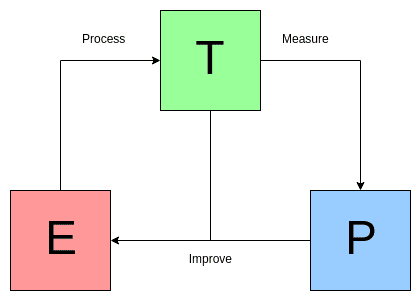
\includegraphics[width=.5\linewidth]{features/etp}
  \caption[机器学习方法的形式化定义]{\label{fig:etp}机器学习的形式化定义}
\end{figure}

尽管机器学习的相关概念早在上世纪五十年代就已经被提出,但直到进入新世纪后,机器学习才真正迎来井喷式发展的黄金期。在过去二十年中,由于半导体电子计算机行业的充分发展,人类收集、传输、处理数据的能力取得了长足的进步,
人类各种社会活动中出现的海量数据具备了能够被挖掘、分析的硬件基础与需要被分析并加以利用的客观需求。在此背景下,机器学习受到了学者们的广泛关注并进入了蓬勃发展阶段,不论是理论基础方面亦或是应用研究方面都
得到了巨大的发展,取得了重大突破。目前,机器学习技术已经被成功应用在模式识别、数据挖掘、自然语言处理、语言识别、图像识别、芯片设计、信息检索及生物信息学等学科领域,
尤其是为交叉学科的发展研究提供了新的技术支撑与突破点\cite{Zhou2016,Aurélien2018,Li2017}。

\subsection{机器学习的分类}
尽管有多种分类标准,基于机器学习在学习阶段呈现的输入数据与预期输出之间的潜在映射关系可将机器学习归纳为以下几类\cite{awad2015,Li2017,Aurélien2018}:

一、监督学习

监督学习是一种用于推断观察数据(也称为输入数据)与目标变量(因变量或标签)之间的潜在关系的学习机制。
学习任务使用标记的训练数据(训练示例)来合成模型函数,这些模型函数的目的是概括特征向量(输入)和监控信号(输出)之间的基本关系。
训练数据包括观察到的输入(特征)向量和期望的输出值(也称为监控信号或类别标签)。基于监督学习算法的经过良好训练的函数模型可以准确预测隐藏在不熟悉或未观察到的数据实例中的隐藏现象的类标签。

二、无监督学习

无监督学习算法被设计用于发现未标记数据集中的隐藏结构,其期望输出是未知的。
一般而言,无监督学习的数据集仅由数据特征集$x_1,x_2,\dots,x_n$组成,没有监督学习中的目标输出,也不包含任何环境激励回报。
聚类与降维是无监督学习两个最为流行的应用方向。此外,无监督学习机制在数据压缩、离群点检测、分类、人类学习等领域均有着广泛应用\cite{awad2015}。

三、半监督学习

半监督学习使用少量标记数据集和大量未标记数据集的组合来生成模型函数或分类器,是监督学习与无监督学习两种机制的结合。
随着海量数据的涌现,对原始数据集的标记过程往往需要大量的人力成本、时间成本,直接对这些数据进行监督学习无疑是不明智的。
而半监督学习正是以未标记的数据为基础,综合应用无监督学习(大量未标记的训练数据)和监督学习(少量标记的培训数据)两种机制,可以显著提高学习精度。
半监督学习目前已在网络数据、消息数据、股票数据、零售数据、生物数据、图像等领域得到应用,特别是在与人类学习相关的语音、视觉和手写识别等领域\cite{awad2015,Aurélien2018}。

四、强化学习

强化学习是通过给定的一组实验动作和观察到的对环境状态的响应进行训练来合成适应模型的过程。
这种方法可以被视为一种控制理论的试错学习范式,其学习系统(在其语境中一般也称为智能体)能够观察环境,做出选择,执行操作,并获得回报或惩罚。
为最大化累计奖励,强化学习的智能体必须自主学习什么是最好的策略。
强化学习在信息论、博弈论、自动控制等领域均得到应用。近年来大热的阿尔法围棋(AlphaGo)就是强化学习最为典型的应用之一\cite{Silver2016}。

五、转换学习

转换学习(又称转换推理)试图通过使用与新案例相关的训练数据集上的额外观察来预测特定测试案例上的排他性模型函数。
转换学习通过将新的个体观测(训练数据)拟合到空间中的单个点来建立局部模型而非全局模型,在给定问题空间出现不连续时有着极佳的发挥空间,可以在不连续边界合成多个模型\cite{Silver2016}。

\section{基本机器学习模型的应用(监督学习)}
本小节对本研究涉及的机器学习中经典监督学习的算法模型进行介绍。

\subsection{决策树}
决策树(Decision Tree,DT)是数据挖掘的经典算法之一,是一种类似流程图的树结构,可以用于连续数值型变量的回归预测及离散型数值型变量的分类问题\cite{Li2017,Liu2018}。
决策树算法的最显著优点是简单直观,易于可视化、可读性强。

一、决策树的结构与原理

分类决策树模型是对实例进行分类的树形结构的描述,如\autoref{fig:dt}所示。一般而言,决策树由结点和有向边组成,而结点又可分为内部结点与叶节点。其中,前者表示一个特征或属性,后者对应决策结果,一般是一个类\cite{Li2017,Zhou2016}。
决策树可以看成一个if-else规则的集合,决策树的根节点到叶节点的每条路径分别对应着一条规则:路径上的内部结点集合构成了规则的判断条件,而叶节点所属的具体类则对应着该规则的结论。
决策树的学习目的就是从训练数据集中集中归纳出一组分类规则,产生一颗与训练数据的矛盾小的、泛化能力强的逻辑判断树。
\begin{figure}[htbp]
    \centering
    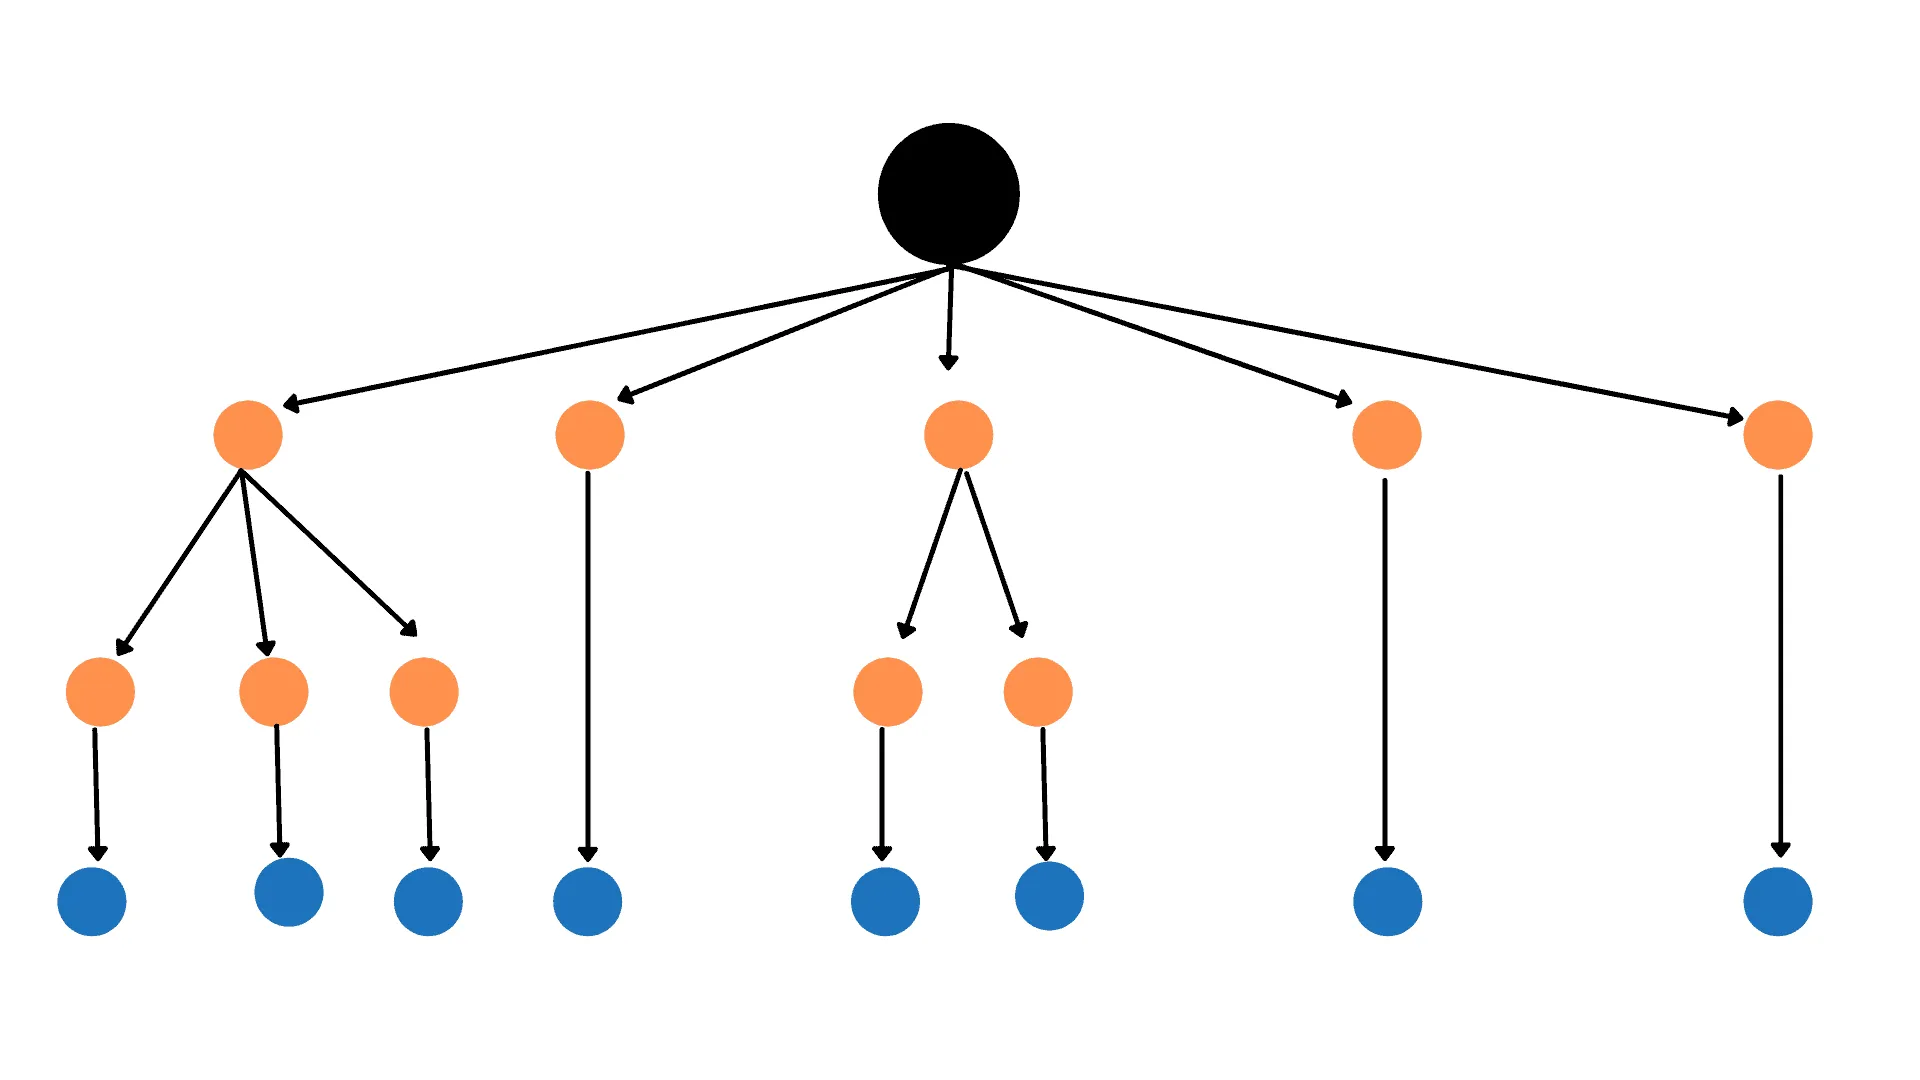
\includegraphics[width=.6\linewidth]{models/dt.png}
    \caption{\label{fig:dt}决策树模型示意}
\end{figure}

二、决策树的特征选择

为生成一颗分类能力强的决策树,一种可行的策略是只选取对分类效果有提升的特征参与构建。基尼指数(Gini index)与信息增益(information gain)是两种最常用的用于筛选最佳特征的指标。

基尼指数,也称为基尼不纯度,其定义为
\begin{equation}
    \label{equ:gini}
    G_i = 1 - \sum_{k=1}^n{p_{i,k}}^2
\end{equation}
其中,$p_{i,k}$是第$i$个节点上,类别为$k$的训练实例占比。基尼指数数值越大,样本集合的不确定性也越大。特别地,若样本集合$D$根据特征$A$是否取某一可能值$a$而被分割成$D_1$和$D_2$两部分,即
\begin{equation}
    \label{equ:daset}
    \left \{
    \begin{aligned}
        D_1 &= \{ (x,y) \in D \mid A(x) = a\} \\
        D_2 &= D - D_1
    \end{aligned}
    \right.
\end{equation}
那么,在特征$A$的条件下,样本集合的基尼指数可以表示为
\begin{equation}
    \label{equ:ginia}
    G(D,A) = \frac{|D_1|}{|D|}G(D_1) + \frac{|D_2|}{|D|}G(D_2)
\end{equation}
其中,$|D|$表示样本集合$D$的样本数量。\autoref{equ:ginia}描述了$D$经特征$A=a$分割后的不确定性,此时,筛选最佳特征的过程可以转换为寻找使\autoref{equ:ginia}取值最小的特征$A$的具体数值。

另一方面,信息增益是在引入了信息论中的信息熵(information entropy)概念进行定义的并计算使用的,其作用与具体使用方法与基尼指数类似,这里不再进行赘述\cite{Zhou2016,Li2017}。

三、决策树的生成

决策树的生成构建过程就是递归地选择最优特征,并根据最优特征对训练数据进行分割,使该分割对各个新的子数据集有最优分类效果的过程。其中,最经典生成算法包括ID3(Iterative Dichotomiser 3,第三代迭代二分器)决策树学习算法、
C4.5(Classifier 4.5,第4.5代分类器)决策树学习算法及CART(classification and regression tree,分类与回归树)决策树学习算法等三种\cite{quinlan1986,quinlan1993,breiman1984}。
在这三种算法中,只有CART算法生成的决策树既可以执行分类任务也可以执行回归任务,故CART算法的应用也最为广泛。

CART算法采用最小基尼指数来选择特征,生成的决策树为二叉树。其工作的基本原理如\autoref{alg:cart}所示。
\begin{breakablealgorithm}
    \caption[CART生成算法]{CART递归生成算法\cite{Li2017}}
    \label{alg:cart}
    \begin{algorithmic}[1] %每行显示行号
        \Require 训练数据集$D$。
        \Ensure CART决策树。
        \State 建立一颗空树$CART$,设该树的根结点为$root$。
        \Function{GenerateCart}{$CART,D_c,root$}
            \State $D_c$为当前结点的训练数据集,计算现有特征对该数据集的基尼指数。对每一个特征$A$,对其可能取的每个值$a$,根据样本点对$A=a$的测试为“是”或“否”将$D_c$分割成$D_l$与$D_r$两部分,使用\autoref{equ:ginia}计算$A=a$时的基尼指数。
            \State 在所有可能的特征$A$以及它们所有可能的切分点$a$中,选择基尼指数最小的特征及其对应的切分点作为最有特征与最优切分点。
            \State 依最优特征与最优切分点,从现结点生成两个子节点$left$与$right$,将训练数据集依特征分配到两个子节点中去,即$D_l$与$D_r$。更新当前$CART$。
            \If {结点中的样本个数小于预定阈值 \textbf{or} 样本集的基尼指数小于预定阈值 \textbf{or} 没有更多特征}
                \State \Return{$CART$}
            \Else    
                \State \Call{GenerateCart}{$CART,D_l,left$}
                \State \Call{GenerateCart}{$CART,D_r,right$}
            \EndIf
        \EndFunction
    \end{algorithmic}
\end{breakablealgorithm}

四、决策树的剪枝

为防止决策树出现过拟合的情况,通常都会对过于“茂密”的树进行剪枝(pruning)处理。决策树的剪枝方法可以分为预剪枝与后剪枝两大类。
前者的工作原理是在决策树的生长阶段就对其进行一定的限制,包括限制树最大生长深度、限制决策树生成的最多叶节点数量等。
后剪枝则是在决策树得到完全生长之后进行,其处理算法也更复杂、训练时间等开销也更大\cite{Zhou2016,Liu2018}。

\subsection{监督学习的其他方法}
除决策树外,常见的无监督学习的算法还包括线性回归算法(linear regression)、随机梯度下降(stochastic gradient descent,SGD)算法、支持向量机(support vector machine,SVM)算法、
K-近邻(K-nearest neighbor,KNN)算法及贝叶斯分类算法(naive Bayes, NB)等\cite{Zhou2016,Li2017,Liu2018,Aurélien2018}。由于篇幅原因,这里对这些算法不作过多介绍。

\section{集成学习的应用}
与此前的诸多算法不同,集成学习(ensemble learning)并不是一个特定的单独机器学习算法,而是使用多种算法构建多个学习器并结合它们的输出完成学习任务的过程\cite{Zhou2016,Aurélien2018}。
集成学习也因此被看成是一种元算法(meta-algorithm),结合多个学习器进行集成学习,通常会获得比单一学习器更好的性能与泛化效果。
\begin{figure}[htbp]
    \centering
    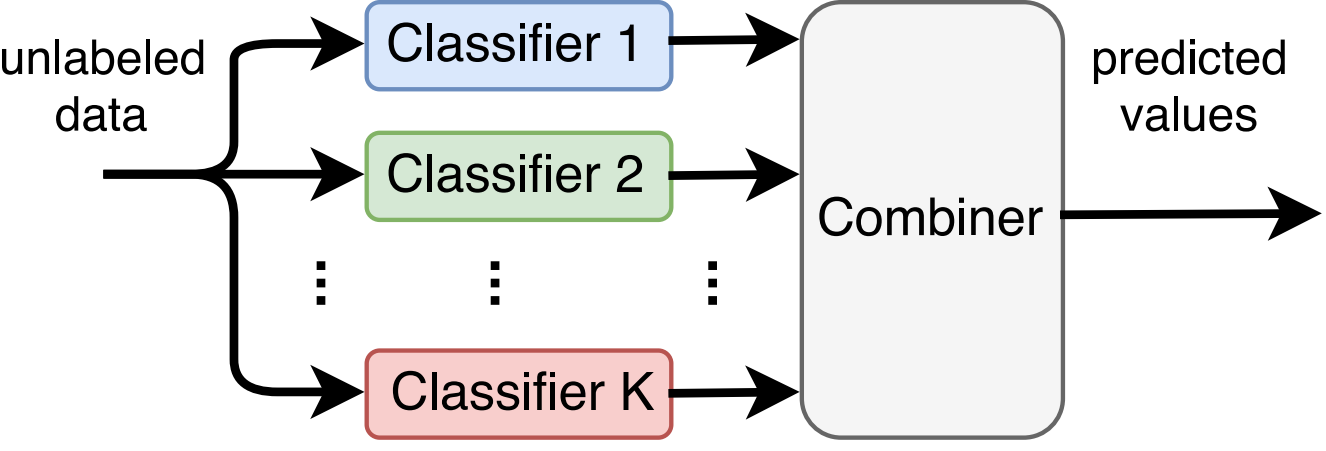
\includegraphics[width=.6\linewidth]{models/el}
    \caption[集成学习示意]{\label{fig:el}集成学习示意}
\end{figure}

一般而言,一个完整的集成学习算法包括构建基学习器与结合基学习器两步,如\autoref{fig:el}所示。其中,按构建方法按个体学习器之间是否存在依赖关系、必须顺序化生成可以分为平行方法与序列化方法两大类\cite{Zhou2016}。
前者的代表是Boosting算法,后者的代表是自举汇聚法(bootstrap aggregating,bagging)与随机森林(Random Forest,RF)。组合基学习器的策略有平均法、投票法及学习法等三类。平均法将各个基学习器按一定的权值累加后作为最终输出
\begin{equation}
    \label{equ:average}
    H(x)=\sum_{i=1}^{T}{w_ih_i(x)}
\end{equation}
其中,$w_i$是个体学习器$h_i$的权值,$w_i\le 0$,$\sum_{i=1}^T{w_i}=1$。

若将多个学习器$h_i$在样本$x$上的预测输出表示为$N$维向量
\begin{equation}
    \label{equ:vector_h}
    \boldsymbol H(x) = [h_1(x),h_2(x),\cdots,h_N(x)]
\end{equation}
其中,$h_i(x)$的值域为类别标记集合$\{c_0,c_1,\cdots,c_N\}$。
此时,上述评估过程可进一步抽象成
\begin{equation}
    \label{equ:output_h}
    Y(x) = f(\boldsymbol H(x))
\end{equation}
其中,$f$为具体决策策略函数。

在机器学习领域,集成学习(参见本研究第5章相关内容)中的投票策略(voting)给出了几种决策方法$f$\cite{Zhou2016}。
具体而言,集成学习将上述学习器$h_i$按输出值类型分为了类标记与类概率等两大类。
而基于这两类输出值进行的投票也相应被称为硬投票与软投票,类标记与类概率的特点可总结概括为\autoref{tab:vote}所示。
其中,硬投票可能会导致最终的分类结果由多数概率值较低的学习器决定,而非少数概率更高、更有分类把握的学习器。因此,在条件允许的情况下,应尽可能使用软投票机制进行决策。
本研究在借鉴集成学习常见可用的三种投票策略的基础上\cite{Kittler1998,Zhou2016},重新设计了更符合PPG检波算法的投票决策机制,以下为具体介绍:
\begin{table}[htbp]
    \centering
    \caption{\label{tab:vote}类标记与类概率特点对比}
    \begin{tabularx}{\linewidth}{c|X<{\centering}X<{\centering}}
        \Xhline{1pt} 
            &\textbf{类标记}&\textbf{类概率}\\
        \hline
        \textbf{$h_i^j(x)$值域}  &$\{0,1\}$    &$[0,1]$     \\
        \textbf{$h_i^j(x)$输出说明}&\tabincell{c}{若$h_i$将样本$x$预测为$c_j$\\则取值为1,否则为0}&\tabincell{c}{$h_i^j(x)$相当于对后验概率\\$P(c_j|x)$的一个估计}\\
        \textbf{投票策略}&\tabincell{c}{绝对多数投票法、\\相对多数投票法}&加权投票法\\
        \textbf{别称}    &硬投票 &软投票 \\
        \Xhline{1pt}
    \end{tabularx}
\end{table}

1.绝对多数投票法

绝对多数投票法的决策原则为若某标记得票数超过半数,则预测为该标记,否则拒绝该预测。
\begin{equation}
    \label{equ:mvoting}
    H(x)=
    \left \{
    \begin{aligned}
        c_j,&\quad if \sum_{i=1}^T{h_i^j(x)}>0.5\sum_{k=1}^N{\sum_{i=1}^T}{h_i^k(x)}\\
        reject,&\quad otherwise.
    \end{aligned}
    \right.
\end{equation}

2.相对多数投票法

应用绝对多数投票法时,若对所有标记类别,其得票数均不超过半数,则此时无法得出投票结果。为避免此情况发生,相对多数投票法直接将预测为得票最多的标记。若同时有多个标记获得最高票,则从中随机选取一个作为最终结果。
\begin{equation}
    \label{equ:pvoting}
    H(x)=c_{\arg \max\limits_{j} \sum_{i=1}^T{h_i^j(x)}}
\end{equation}

3.加权投票法

与前面两种投票法不同,加权投票法给所有的学习器$h_i$以特定的权重$w_i$,将所有可能汇总后得到最后的标记类别,
\begin{equation}
    \label{equ:wvoting}
    H(x)=c_{\arg \max\limits_{j} \sum_{i=1}^T{w_ih_i^j(x)}}
\end{equation}
其中,$w_i\ge0$,$\sum_{i=1}^T{w_i=1}$。
投票法是从多个个体学习器的结果中票选出结果,相关概念已经在本文第三章介绍脉搏波检测算法时进行过介绍,在此不再赘述。而学习法则是使用额外的学习器来完成基学习器的结果输出。

\subsection{Bagging与随机森林}
一、Bagging

为获得泛化性能强的不同的基学习器,一种可行的策略是对所有学习器使用同一种训练算法,但是在训练集的不同随机子集上进行训练,使这些基学习器的能够有一定的差异。
\autoref{fig:bp}所示,在上述过程的随机子集的建立过程中,若对原始数据样本的采样后放回,这种方法即为bagging;与之对应的,采样后不放回的方法称为pasting\cite{Aurélien2018,Zhou2016}。
由于bagging方法可以获得的随机子集数量要远远高于pasting方法,bagging方法应用得也更加广泛。
\begin{figure}[htbp]
    \centering
    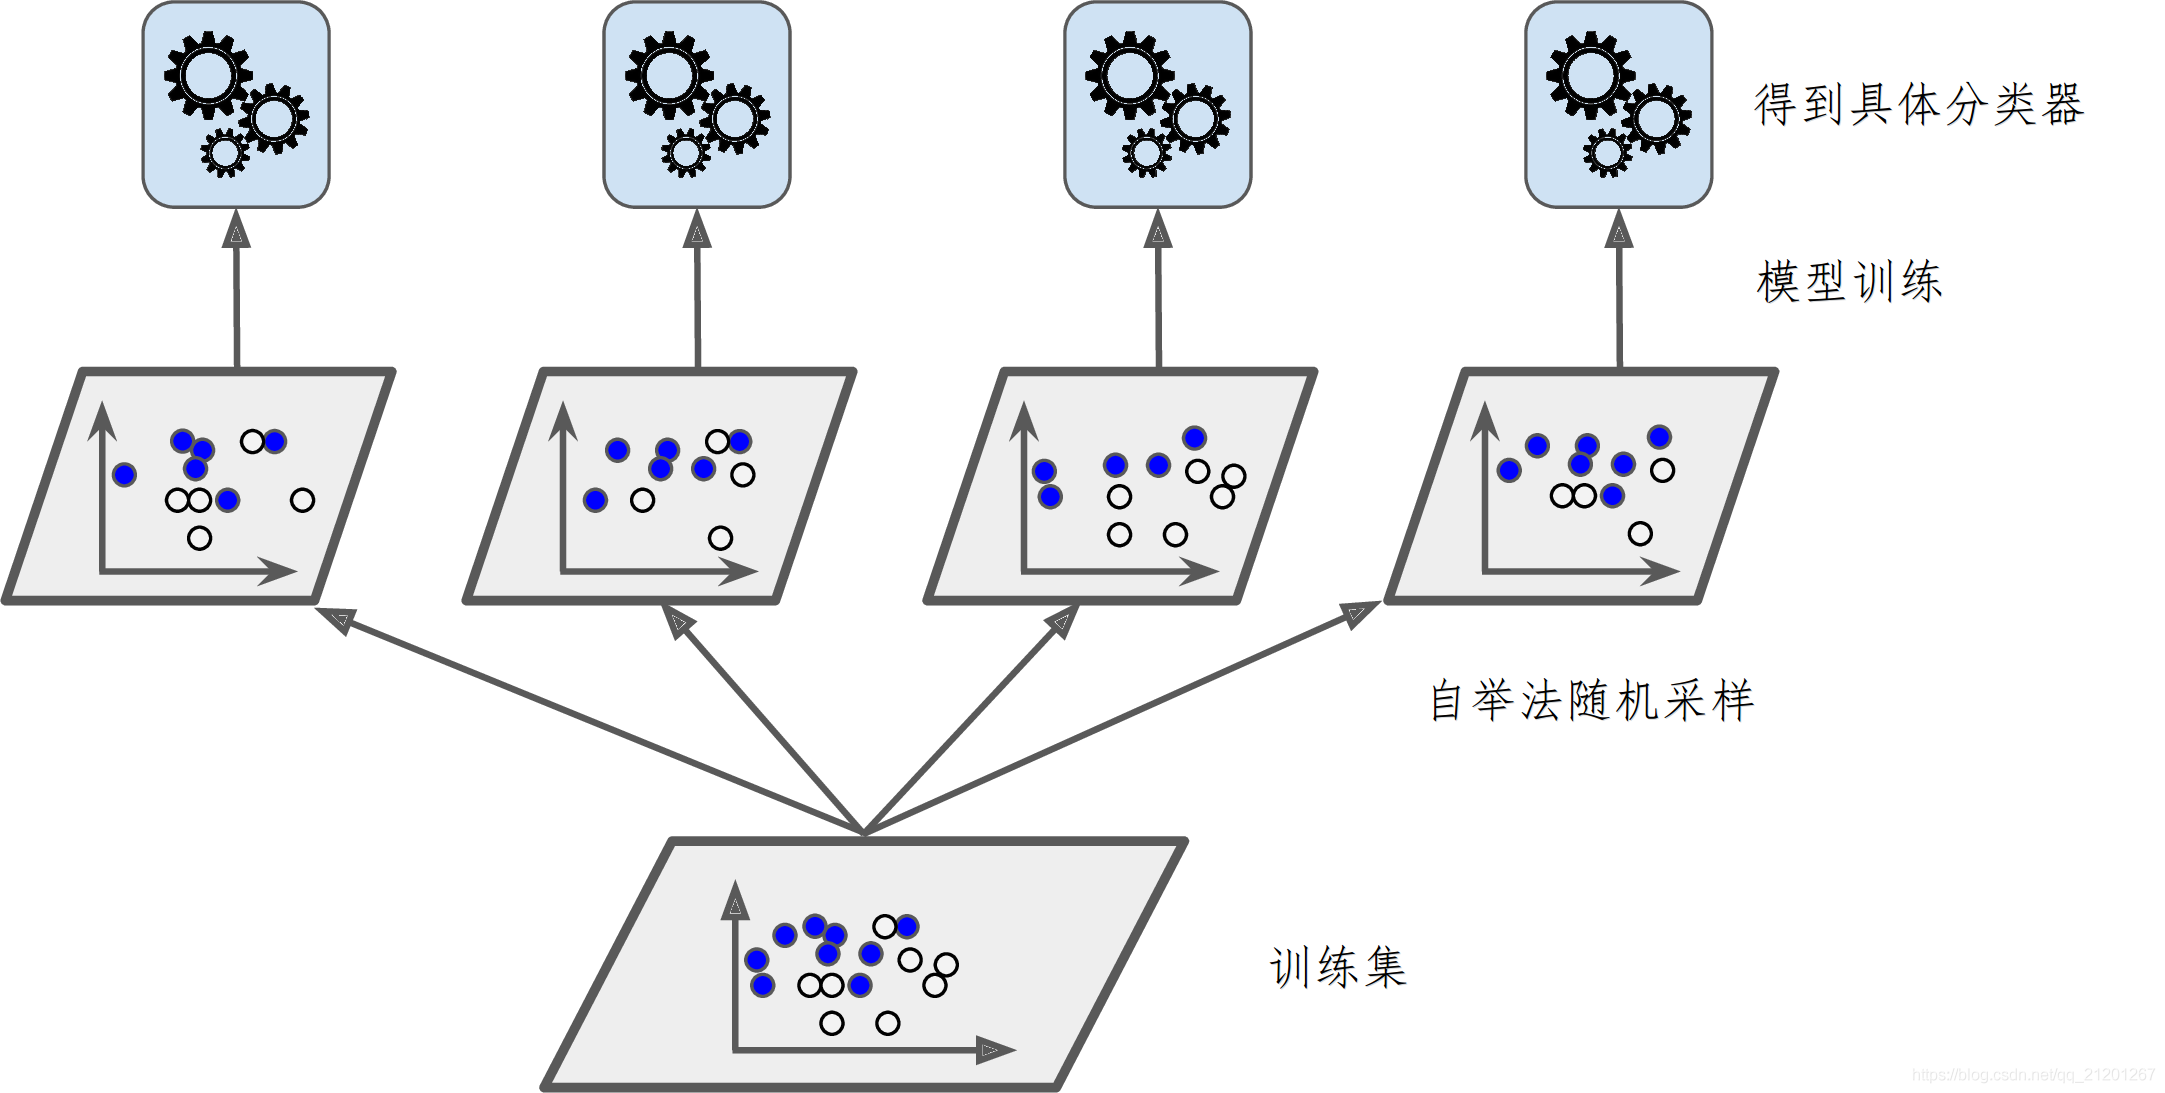
\includegraphics[width=.6\linewidth]{models/bp}
    \caption[Bagging与Pasting示意]{\label{fig:bp}Bagging与Pasting示意\cite{Aurélien2018}}
\end{figure}

当使用有采样后即放回的方法从包含$m$个原始样本的训练集$D$抽取出$m$个新的样本构成此次训练数据集$D_{bs}$时,显然,$D$有部分数据样本在$D_{bs}$重复出现,部分数据则从未被抽样过。
易知样本在$m$次均未被抽中的概率为$(1-\frac{1}{m})^m$,当$m \to \infty$时,
\begin{equation}
    \label{equ:me}
    \lim_{m \to \infty}{(1-\frac{1}{m})}^m = \frac{1}{e} \approx 0.368
\end{equation}
\autoref{equ:me}说明约有36.8\%的原始样本未出现在采样集$D_{bs}$中,这部分数据可以作为当前训练算法的测试集。

按上述思想,可从原始样本训练集$D$采样得到$T$个包含$m$个训练样本的采样集,基于这些采样集,使用特定的机器学习算法可以训练得到$T$个基学习器,结合这些基学习器的输出即为Bagging算法
的基本流程,如\autoref{alg:bagging}所示。投票法和平均法是Bagging在进行基学习器的输出时常采用的策略。
\begin{breakablealgorithm}
    \caption[Bagging算法]{Bagging算法\cite{Zhou2016}}
    \label{alg:bagging}
    \begin{algorithmic}[1] %每行显示行号
        \Require 训练集$D=\{(x_1,y_1),(x_2,y_2),\dots,(x_m,y_m)\}$;基学习算法$\xi$;训练轮数$T$。
        \Ensure $H(x)=\arg \max \limits_{y \in Y} \sum_{t=1}^T \mathbb{I}(h_t(x)=y)$,其中$\mathbb{I}(.)$为指示函数,在$.$为真或假时函数值分别为1或0。
        \For {$t=1,2,\dots,T$}
            \State 从原始训练集$D$自助采样得到此次的样本分布$D_{bs}$
            \State $h_t=\xi (D,D_{bs})$
        \EndFor
    \end{algorithmic}
\end{breakablealgorithm}

二、随机森林

随机森林是另一种在Bagging算法基础上发展起来的集成学习的算法,最早由Leo Breiman于2001年提出\cite{breiman2001}。如\autoref{fig:rf}所示,“森林”表示该算法是由多棵\autoref{fig:dt}所示的决策树构成,
这些决策树一般都是经过充分生长的、未经剪枝处理的CART决策树。而“随机”一词有两重含义,首先是同Bagging算法一样,每棵决策树在训练时使用的训练样本是随机抽取的;其次,与\autoref{alg:cart}所示的一般CART决策树生成算法不同,随机森林中的CART
决策树在生长时并不是在当前结点的$d$个属性集合$A$中选取最优特征及其最优切分点,而是先从$A$中随机生成一个包含$k$个属性子集的$A_{bs}$,随后再从$A_{bs}$中选择最优属性进行划分\cite{Zhou2016,Liu2018,breiman2001}。其中,$k$的推荐取值为
$\lfloor \log_2m + 1 \rfloor$\cite{breiman2001}。

\begin{figure}[htbp]
    \centering
    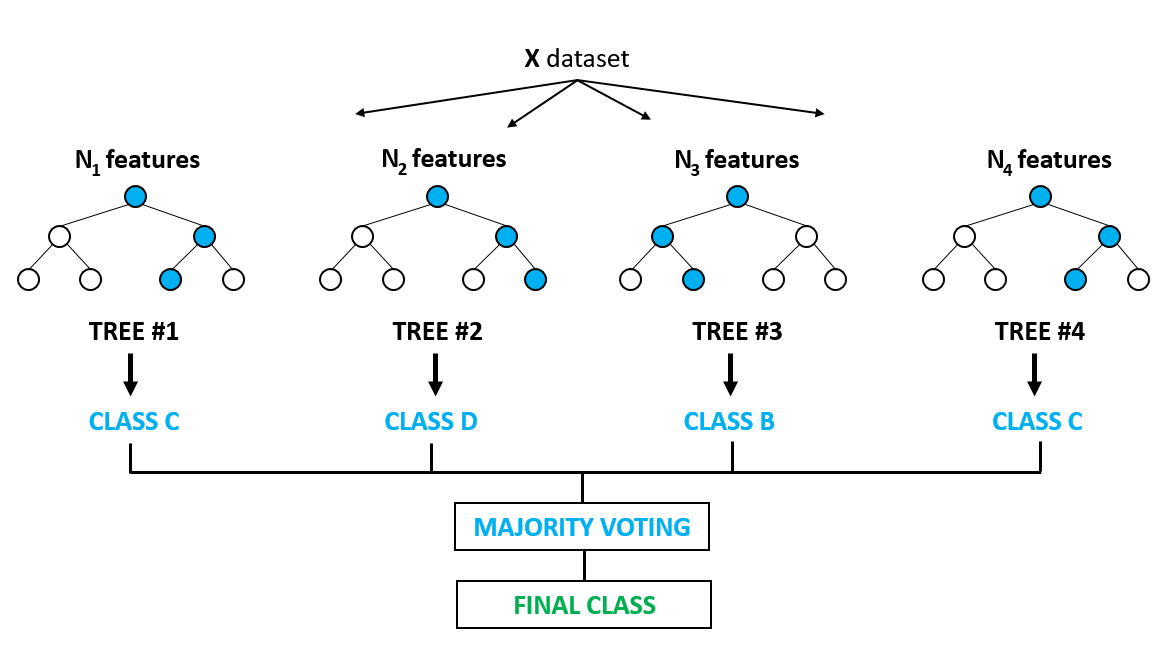
\includegraphics[width=.6\linewidth]{models/rf}
    \caption{\label{fig:rf}随机森林示意}
\end{figure}

对回归问题而言,随机森林算法的输出是所有决策树的输出的均值;而对分类任务而言,算法输出是所有决策树输出投票的结果。随机森林在树的生长过程中的两次随机使决策树具有更大的多样性,相当于用更高的偏差换取更低的方差。因此,
最终的集成结果有着出色的泛化性能,有效避免了单决策树可能导致的过拟合问题。随机森林算法运行速度快、准确率高且泛化性能优秀,被誉为“代表集成学习技术水平的方法”\cite{Zhou2016,Liu2018}。

此外,随机森林算法往往也会在特征选择的过程中得到应用\cite{Aurélien2018}。重新考察\autoref{fig:dt}中的决策树可以发现,越靠近根结点位置的特征对决策过程的重要程度也越高,而不重要的特征多出现在靠近结点的位置、甚至不出现在决策树中。
因此,特征的重要性(或贡献度)可以通过计算其在随机森林众多决策树的平均深度来进行量化衡量。

\subsection{堆叠法}
此前已经介绍过学习法是一种使用额外的学习器来完成多个基学习器的结果输出策略。相较平均法与投票法这种简单策略,学习法有着更为强大的性能优势。而堆叠法(Stacking)则是学习法中最为典型的代表。其中,基学习器也称为初级学习器,用于
结合的学习器称为次级学习器或元学习器(meta-learner),如\autoref{fig:stacking}所示。

\begin{figure}[htbp]
    \centering
    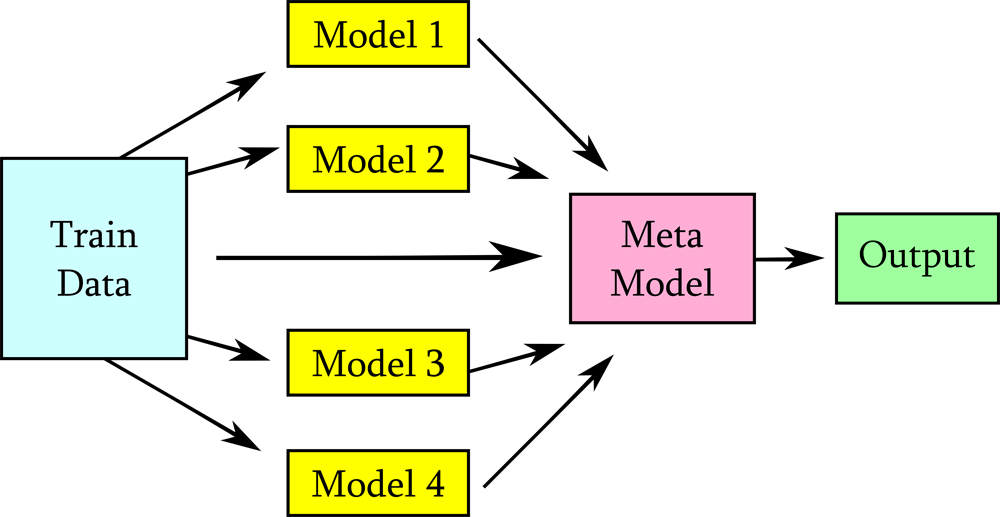
\includegraphics[width=.6\linewidth]{models/stacking}
    \caption{\label{fig:stacking}堆叠法原理示意}
\end{figure}

在使用堆叠法时,需要先从初始数据集中训练出多个初级学习器,然后“生成”一个新数据集用于训练次级学习器。多个初级学习器是同质或异质均可,即使用相同或不同学习算法产生。
在新生成的数据集中,初级学习器的输出作为新样本的输入特征,而对应的初始样本的标记仍被当做新样本的标记。整个堆叠法的算法描述如\autoref{alg:stacking}所示。
\begin{breakablealgorithm}
    \caption[堆叠算法]{堆叠算法\cite{Zhou2016}}
    \label{alg:stacking}
    \begin{algorithmic}[1] %每行显示行号
        \Require 训练集$D=\{(x_1,y_1),(x_2,y_2),\dots,(x_m,y_m)\}$;初级学习算法$\xi_1,\xi_2,\dots,\xi_T$;次级学习算法$\xi$。
        \Ensure $H(x)=h^{'}(h_1(x),h_2(x),\dots,h_T(x))$。
        \For {$t=1,2,\dots,T$}
            \State 使用初级学习算法$\xi_t$训练产生初级学习器$h_t$。
            \State $h_t=\xi_t (D)$
        \EndFor
        \State $D^{'}=\emptyset$
        \State 生成次级训练集
        \For {$i=1,2,\dots,m$}
            \For {$t=1,2,\dots,T$}
                \State $z_{it}=h_t(x_i)$
            \EndFor
            \State $D^{'}=D^{'} \cup ((z_{i1},z_{i2},\dots,z_{iT},),y_i)$
        \EndFor
        \State $h^{'}=\xi(D^{'})$
    \end{algorithmic}
\end{breakablealgorithm}

\section{基本机器学习模型的应用(无监督学习)}
与监督学习类算法相比,无监督学习算法由于不需要任何数据标签,且在训练学习时不需对原始数据的分布作过多要求,因此,无监督学习算法也逐渐称为一个新的研究热点。
聚类(clustering)是无监督学习算法中最为典型的应用之一,本小节将介绍几种有代表性的聚类算法。

\subsection{K均值}
K均值(K-Means)算法属于原型聚类算法的一种\cite{Zhou2016,Liu2018}。顾名思义,该算法可以将原始数据$D=\{x_1,x_2,\dots,x_n\}$划分为指定的K个簇$C=\{C_1,C_2,\dots,C_n\}$,并使得平方误差最小化
\begin{equation}
    \label{equ:leastsq}
    E=\sum_{i=1}^k \sum_{x \in C_i}{||x- \mu_i||}_2^2
\end{equation}
其中,$\mu_i = \frac{1}{|C_i|} \sum_{x \in C_i}{x}$是簇$C_i$的均值向量。

\autoref{equ:leastsq}反应了各簇内样本整体相似度,同时也反应了簇内样本围绕均值向量的紧密程度。一般而言,$E$的数值越小,簇内样本相似度越好,此次聚类的效果越好。
\autoref{alg:kmean}给出了K均值算法的工作原理。\autoref{fig:kmeans}则给出了一个具体的使用K均值算法进行聚类的过程示意。
\begin{breakablealgorithm}
    \caption[KMeans聚类算法]{KMeans聚类算法\cite{Zhou2016}}
    \label{alg:kmean}
    \begin{algorithmic}[1] %每行显示行号
        \Require 样本集$D=\{x_1,x_2,\dots,x_m\}$,聚类簇数$k$。
        \Ensure 簇划分$C=\{C_1,C_2,\dots,C_k\}$
        \State 从D中随机选择k个样本作为初始均值向量$\{\mu_1,\mu_2,\dots,\mu_k\}$
        \Repeat
        \State 令$C_i=\emptyset (1\le i\le k)$
            \For {$j=1,2,\dots,m$}
                \State 计算样本$x_j$与各均值向量$\mu_i (1\le i \le k)$的距离:$d_{ij}={||x_j - \mu_j||}_2$
                \State 根据距离最近的均值向量确定$x_j$的簇标记:$\lambda_j = \arg \min_{i \in \{1,2,\dots,k\}} d_{ij}$
                \State 将样本$x_j$划入对应的簇:$C_{\lambda_j} = C_{\lambda_j} \cup \{x_j\}$
            \EndFor
            \For {$i=1,2,\dots,k$}
                \State 计算新均值向量:$\mu_i^{'}=\frac{1}{|C_i|} \sum_{x \in C_i}{x}$
                \If {$\mu_i^{'} \ne \mu_i$}
                    \State 将当前均值向量$\mu_i$更新为$\mu_i^{'}$
                \Else
                    \State 保持当前均值向量不变
                \EndIf
            \EndFor
        \Until 当前均值向量均未更新
    \end{algorithmic}
\end{breakablealgorithm}
\begin{figure}[htbp]
    \centering
    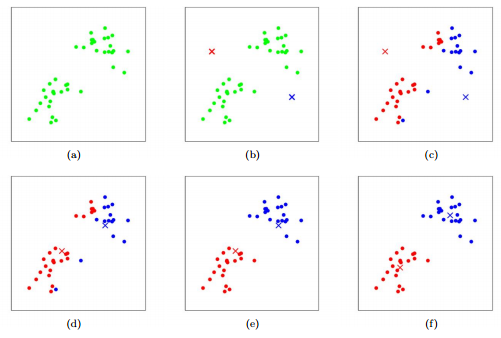
\includegraphics[width=.6\linewidth]{models/kmeans}
    \caption[Kmeans算法运行示意]{\label{fig:kmeans}Kmeans算法运行示意\cite{kmeans}。训练样本显示为点,簇中心向量显示为$\times$。(a)为原始数据集。(b)给出了两个随机的簇中心向量。(c-f)每两次迭代运行K均值算法后的聚类效果。}
\end{figure}

\subsection{无监督学习的其他方法}
除K近邻算法外,原型聚类算法还包括学习向量量化(Learning Vector Quantization,LVQ)算法、高斯混合聚类(Mixture of Gaussian)算法等。此外,密度聚类(density-based clustering)与层次聚类
(hierarchical clustering)则是按照另外的标准对原始数据样本分簇的算法。具有噪声的基于密度的聚类(Density-Based Spatial Clustering of Applications with Noise,DBSCAN)算法
与自底向上层次聚类(Agglomerative Nesting,AGNES)算法分别是两者的典型代表\cite{Zhou2016}。

\section{深度学习模型的应用}
\section{小结}
本研究过程中基于脉搏波特征数据,综合使用了多种机器学习模型算法进行了子痫前期的识别模型建立。而本章则从这些模型中选取了最为经典几种算法进行了原理性的介绍说明。
